\chapter{O Projeto}
\label{chapter:projeto}

Devido a interação entre dispositivos de aquisição de dados e os de aplicação e armazenamento de dados em diferentes cenários (como descrito em \ref{section:overview}), foi necessário uma implementação de um protocolo de comunicação entre os dispositivos em diferentes linguagens de programação.

A arquitetura Publish/Subscribe define as configurações gerais do sistema, não contempla as mudanças de cenário possíveis, onde , por exemplo, a rede esteja congestionada e é necessário tomar medidas como reduzir a taxa de dados que são enviados em tempo real. É necessária a adição de configurações dinâmicas que se adaptem as condições impostas pelos cenários, uma interface que varia com as condições de cada par Publisher/Subscriber formado. Para isso, foi criado o conceito de Data Stream.

O protocolo consiste em configurações de uma abstração de um canal de envio de dados chamado Data Stream mostrado em \ref{fig:3.1.0/data_stream}, no qual transitam dados em uma determinada velocidade, podendo conter um limite de pacote de dados. Nas pontas desse canal estão os Publishers e Subscribers, descritos na seção \ref{subsection:publishers_subscribers}. Este conceito permite  que a interface possa reagir a limitações de transmissão, como congestionamento na rede. O desenvolvedor irá se preocupar somente com as configurações do canal.


\section{Data Streams}
\label{section:data_stream}

Um Data Stream é uma parte da interface que permite adicionar configurações de como o dado será enviado pelo Publisher  para lidar com problemas na transmissão, como o próprio cenário de congestionamento da rede já citado. As configurações podem ser enviadas (ou alteradas) pelo Subscriber, permitindo configurações dinâmicas para o Data Stream utilizado na transmissão. A configuração pode lidar com qualquer aspecto do envio de dados, como o tamanho das mensagens enviadas, ou a taxa de envio ou no próprio formato de mensagem.


Publishers são dispositivos que criam Data Stream  e enviam dados por estes, regulam o processamento dos dados, estipulam limites de tamanho de cada pacote de dado e determinam o intervalo de envio de pacotes. O protocolo permite que os Publishers enviem os dados e também permite que outros dispositivos possam passar configurações remotamente para modificar os parâmetros de cada Data Stream, como o intervalo de envio ou a adição de um novo parâmetro (como um limite de dados por mensagem, por exemplo) a ser adicionado a configuração. 

\begin{figure}[h!]
\centering
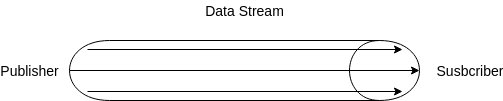
\includegraphics[width=13cm]{./02_Capitulos/02_Cap3/figures/data_stream}
\caption{O conceito de Data Stream para a abstração do transporte de dados}
\label{fig:3.1.0/data_stream}
\end{figure}

Para criar um Data Stream, basta um Subscriber estar assinando um tópico no formato abaixo. E um Publisher publicar neste tópico, como na \ref{fig:3.1.0/data_stream_creation}. O Id corresponde a uma identificação única que pode ser definida pelo desenvolvedor. O \textit{stream\_nome} corresponde ao tipo de Data Stream utilizado, que serão detalhados a seguir.

$$ /\{data\_stream\_id\}/stream:\{stream\_nome\} $$

Existem dois tipos de Data Stream já implementados nos Publishers. Porém o desenvolvedor pode implementar seus próprios Data Streams dependendo da linguagem de programação utilizada, logo existem três tipos de Data Stream definidos:

\begin{itemize}
\item Contínuo: Data Stream padrão sem configurações definidas que publica continuamente dados;
\item Periódico: Publica dados esperando um período T que pode ser alterado ;
\item Customizáveis: Criados pelo desenvolvedor, com suas próprias configurações.
\end{itemize}

Os Subscribers podem alterar as configurações específicas de cada tipo de Data Stream, baseada nas necessidades da aplicação, como problemas de processamento ou congestionamento na rede etc.

\begin{figure}[h!]
\centering
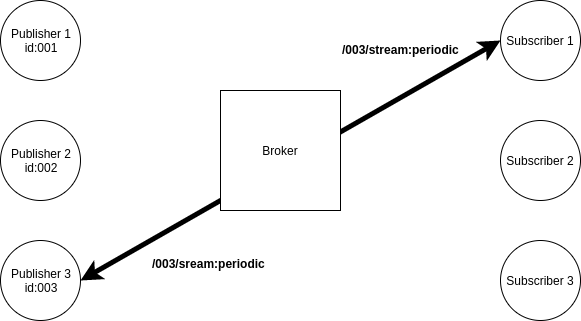
\includegraphics[width=13cm]{./02_Capitulos/02_Cap3/figures/data_stream_creation}
\caption{Um Data Stream é criado a partir do tópico \textit{/003/stream:periodic}}
\label{fig:3.1.0/data_stream_creation}
\end{figure}


Para um Subscriber enviar configurações basta publicar no tópico abaixo. As configurações são feitas por uma string JSON \cite{json}, um conjunto de chaves-valor universalmente interpretada por várias linguagens de programação como forma de transporte de objetos de uma classe. 

$$ /\{data\_stream\_id\}/configure/stream:\{stream\_nome\} $$

A \ref{fig:3.2.0/pub_sub} descreve um cenário onde um Publisher e um Subscriber estão transmitindo dados por um Data Stream pelo tópico textit{/003/stream:periodic}, as setas indicam que o Publisher pode enviar dados para um Subscriber por um Data Stream do tipo \textit{Periódico} com Id \textit{003}, assim como o Subscriber pode enviar alterações nos parâmetros de configuração deste tipo de Data Stream, como o próprio período.


\begin{figure}[h!]
\centering
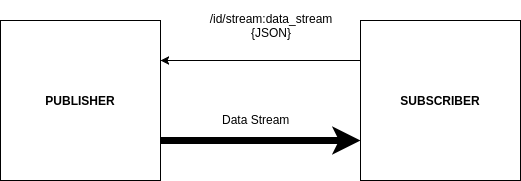
\includegraphics[width=12cm]{./02_Capitulos/02_Cap3/figures/publisher-subscriber_comm}
\caption{Uma outra representação da comunicação entre Publishers e Subscribers por Data Stream}
\label{fig:3.2.0/pub_sub}
\end{figure}


\section{Implementação em Plataformas}
\label{subsection:plataformas}

A camada de aquisição apresenta a implementação dos Publishers, que enviam os dados. As plataformas possuem unidades de processamento e módulos de rede e se comunicam com sensores, para coletar dados físicos, e atuadores que recebem instruções para a execução de alguma função, como abrir/fechar alguma porta ou compartimento, ou ligar alguma iluminação e acionamentos em geral.

\subsection{Sistemas Embarcados}
\label{subsubsection:embarcados}

Sistemas Embarcados, são sistemas alimentados por baterias, sem alimentação de rede elétrica, portáteis, econômicos, com sistemas de controles geralmente feitos por micro-controladores ou microprocessadores, podendo contemplar sistemas operacionais simples. Com essa descrição, pode-se imaginar que estes dispositivos possuem processamento, energia e desempenho limitados. Neste caso, foi necessário a criação de uma implementação de interface leve, que não consuma muito armazenamento e processamento do sistema embarcado, e eficiente no consumo de energia.

Foram escolhidas para a implementação em embarcados as plataformas microcontroladas com arquitetura Espressif \cite{espressif}, como a arquitetura ESP32 que contempla MCUs(Micro-Controller Units), módulos WiFi, sensores internos, entradas e saídas analógicas e digitais e até Bluetooth (não utilizado na versão atual), mostrados na \ref{fig:3.3.4/esp32-arch}. Pela descrição técnica pode-se ver um poder de processamento maior que um Arduino \cite{arduino}, muito utilizado nessas aplicações e que também é compatível com a interface se adicionado shields WiFi. O ESP utiliza linguagem C++ \cite{c++} com framework Arduino para implementar os Publisher e os Data Stream contidos neles no ESP32.

\begin{figure}[h!]
\centering
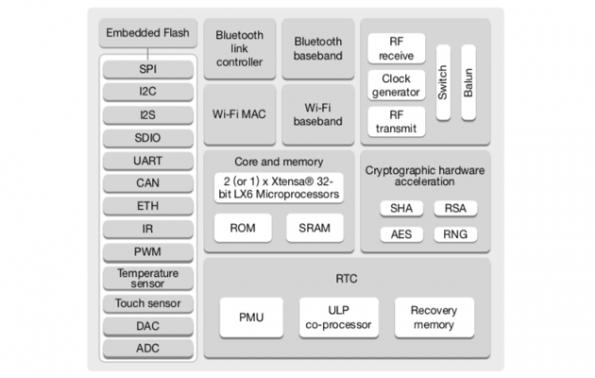
\includegraphics[width=13cm]{./02_Capitulos/02_Cap3/figures/espressif32-arch}
\caption{A arquitetura do ESP32, retirado de \cite{espressif}}
\label{fig:3.3.4/esp32-arch}
\end{figure}


Também foram implementadas, em Javascript  utilizando Node.js \cite{nodejs}, aplicações do Publisher para embarcados com sistemas operacionais, como Raspberry Pi \cite{raspberry-pi}. Permitindo multi-uso entre as funções de Publisher e Subscriber. Esses embarcados mais robustos possuem processadores mais potentes, módulos de rede, sistemas operacionais, entradas e saídas digitais entre outros.


\subsection{Consoles}
\label{subsubsection:consoles}

Consoles são sistemas que contemplam sistemas operacionais, o que permitem mais liberdade para a implementação da interface. Foi escolhida então, realizar a implementação com Node.js um interpretador de Javascript que permite criar aplicações sem a necessidade de usar um browser para interpretar Javascript, como interfaces de linha de comando, aplicações Desktop, entre outros processos permitidos no Sistema operacional. Node.js possui extensas bibliotecas para HTTP e MQTT além de pipelines que permitem fácil comunicação de protocolos e transição de dados no mesmo processo.


\begin{figure}[h!]
\centering
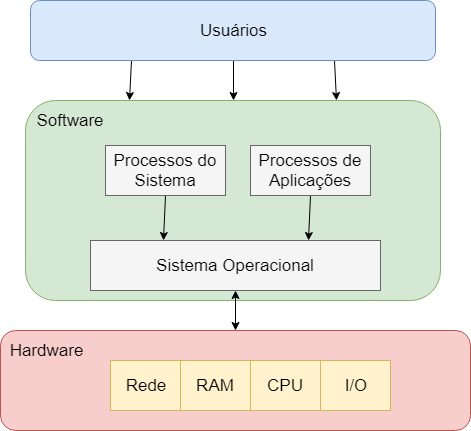
\includegraphics[width=10cm]{./02_Capitulos/02_Cap3/figures/os-diagram}
\caption{A arquitetura simplificada de dispositivos com Sistema Operacional}
\label{fig:3.3.4/os-diagram}
\end{figure}


Além disso, Node.js é uma ferramenta multi-plataforma, com distribuições para Windows, Linux e MAC, além de versões para embarcados de arquitetura ARM, como o próprio Raspberry Pi. Possui Módulos que permitem acessar processos do sistema operacional como ilustrado na \ref{fig:3.3.4/os-diagram} permitindo acesso a Rede além de informações do próprio sistema. O ambiente permite a implementação com programação orientada a objeto, Publishers, Data Streams, Subscribers, são instâncias de classes mostradas no apêndice em \ref{section:codigos_fonte}, permitindo que a aplicação seja feita em um processo (obs: este processo pode executar outros processos, com algum overhead), diminuindo a complexibilidade do sistema, evitando a necessidade de comunicação inter-processos (IPC).  Com isso foram implementadas bibliotecas que constroem a interface sobre o MQTT.

\section{Arquiteturas e Assíncronismo}
\label{section:arquitetura}

Na seção anterior foi discutido a implementação em Hardware do sistema e as diferenças das tecnologias contempladas. Sistemas embarcados 
possuem muito menos funcionalidades que um console gerido por um sistema operacional, sendo uma das principais o paralelismo de processos, a capacidade de ser multi-tarefas Por isso exigiram-se duas filosofias diferentes de implementação do sistema para os dois tipos de plataformas.

\subsection{Arquitetura síncrona em embarcados}
\label{subsection:embarcados_sinc}

Sistemas embarcados possuem um poder de processamento limitado, apesar da tendência de desenvolver embarcados mais potentes. Estes sistemas são geralmente Micro-controlados, ou seja, com arquiteturas mais simples, geralmente executando instruções de somente um programa compilado para linguagem do MCU e gravado neste. Não há paralelismo, cada instrução é síncrona, ou seja, são executadas uma a uma, pela unidade de processamento.

\begin{figure}[h!]
\centering
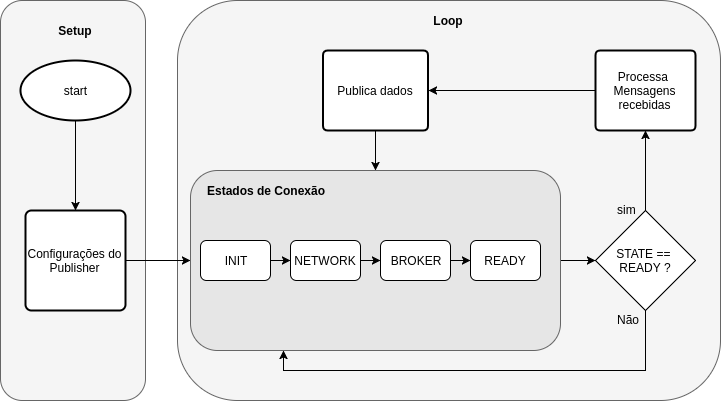
\includegraphics[width=12cm]{./02_Capitulos/02_Cap3/figures/sinc_implementation}
\caption{Diagrama simplificado de uma rotina padrão seguida pela implementação em Microcontroladores}
\label{fig:sinc-implementation}
\end{figure}

A \ref{fig:sinc-implementation} simplifica a lógica da implementação em dispositivos síncronos como micro-controladores. No Apêndice deste documento pode-se encontrar as implementações em C++. O programa começa configurando o objeto Publisher (MQTT) com configurações de conexão a rede e o broker, além de outras definições do desenvolvedor. O bloco de loop repete-se indeterminadamente, verificando o estado de conexão da aplicação que passa pelos seguintes estados:

\begin{itemize}
\item INIT: Estado inicial, verifica conexão com rede;
\item NETWORK: Tem conexão com rede, verifica conexão com Broker;
\item BROKER: Tem conexão com Broker, inicia configurações dos Data Streams;
\item READY: Pronto para enviar e receber mensagens !
\end{itemize}

Quando o estado está em READY, a aplicação está pronto para processar mensagens recebidas e publicar, lembrando que está é uma lógica básica, o desenvolvedor pode adicionar outros passos, mas a verificações de estado e as configurações do Publisher são obrigatórias para o funcionamento do Sistema. Repare que toda a lógica é sequencial, síncrona, não há paralelismo na rotina.

\subsection{Processos assíncronos em console}
\label{subsection:consoles_assinc}

Consoles são dispositivos que possuem uma Arquitetura mais complexa, consequentemente mais poder de processamento. Na \ref{fig:3.3.4/os-diagram}, a presença de um sistema operacional gerenciando processos do sistema e de aplicações e informações do Hardware, permitem a execução de múltiplas tarefas em paralelo, o que caracteriza processos assíncronos. O interpretador Node.js possui uma gama de bibliotecas para a implementação de funções assíncronas, diferentemente dos Sistemas Embarcados microcontrolados, que executa Threads em paralelo, para receber e enviar mensagens simultaneamente.


\begin{figure}[h!]
\centering
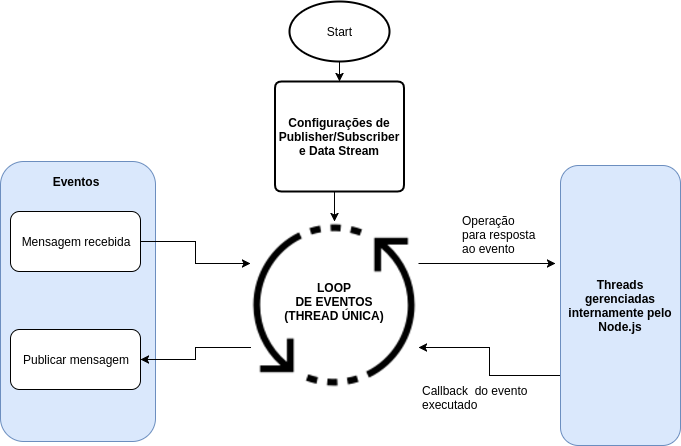
\includegraphics[width=13cm]{./02_Capitulos/02_Cap3/figures/async-implementation}
\caption{Diagrama simplificado de uma rotina assíncrona padrão em Consoles}
\label{fig:async-implementation}
\end{figure}

A \ref{fig:async-implementation} mostra o funcionamento simplificado das aplicações de Publisher e Subscriber em Node.js. A aplicação faz as configurações específicas de cada objeto Publisher ou Subscriber e logo após entra em um Loop de eventos, onde existem eventos de Conexão com a rede e com o Broker, e de envio/recebimento de mensagens, entre outros. Estes eventos quando são acionados pelo sistema, executam callbacks, funções assíncronas definidas e associadas a um evento. Esses callbacks são gerenciados internamente pelo Node.js e direcionadas ao loop de eventos.

\section{Indexação de dados e Timestamp}
\label{section:timestamp}

Na seção, \ref{section:bancos_IoT} foram discutidos estruturas da organização de dados e o formato de armazenamento de dados como o formato de documento e séries de tempo. É importante que estes formatos tenham formas eficientes de indexação, de modo a facilitar a busca e a análise de dados.

Em uma aplicação de IoT, que envolve coleta de dados em tempo real, é fundamental, independentemente do formato escolhido, a data e hora da coleta do dado. Isto permite a análise dos dados ao longo do tempo. Aplicações de decisão e análise utilizam ferramentas estatística com base nas ocorrências temporais, projetando previsões e classificação. No projeto atual, foi implementado o MongoDB, que é um banco de dados de documentos. Cada documento é indexado por uma identificação única como mostrado na \ref{fig:document-model}, permitindo também criar relações entre documentos.

\begin{figure}[h!]
\centering
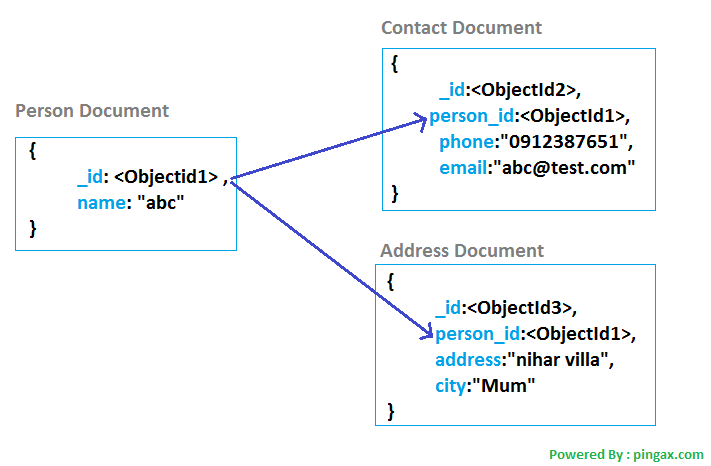
\includegraphics[width=10cm]{./02_Capitulos/02_Cap3/figures/document-model}
\caption{O formato de documento no MongoDB}
\label{fig:document-model}
\end{figure}

O banco também permite adicionar outros parâmetros de indexação definidos pelo desenvolvedor, como o Timestamp, uma informação de data e hora da inserção no banco. Na implementação foi utilizado o formato Unix Timestamp, o número de milisegundos que se passaram desde 1 de Janeiro de 1970 ás 00:00:00 (UTC). A \ref{fig:document-timestamp} ilustra o formato de documento completo usado no sistema, o campo de dados é definido pelo desenvolvedor. 

\begin{figure}[h!]
\centering
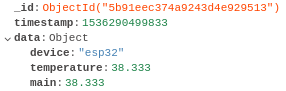
\includegraphics[width=8cm]{./02_Capitulos/02_Cap3/figures/document-timestamp}
\caption{Adição de parâmetro de timestamp em milisegundos ao documento}
\label{fig:document-timestamp}
\end{figure}

Vale ressaltar a existência de uma nova geração de Bancos de Dados de séries de tempo, um formato parecido com o de Documento, porém com indexação feita por Timestamp ao invés de uma chave única. Em destaque o Banco InfluxDB, que possui estrutura LSM-Tree além de ser um banco de séries de tempo, o que o faz ser utilizado cada vez mais em aplicações IoT.